\documentclass{article}

\usepackage[portuguese]{babel}
\usepackage[utf8]{inputenc}
\usepackage[letterpaper,top=2cm,bottom=2cm,left=3cm,right=3cm,marginparwidth=1.75cm]{geometry}
\usepackage{amsmath}
\usepackage{graphicx}
\usepackage[colorlinks=true, allcolors=blue]{hyperref}
\usepackage{listings}
\usepackage{xcolor}
\usepackage{cite}
\usepackage{float}
\usepackage{lipsum}
\usepackage{tabularx}


\lstset{
  language=Python,
  basicstyle=\ttfamily\small,
  numbers=left,
  numberstyle=\tiny\color{gray},
  keywordstyle=\color{blue},
  commentstyle=\color{gray},
  stringstyle=\color{orange},
  breaklines=true,
  frame=single,
  columns=flexible
}

\title{Avaliação 2 de Introdução a Computação}
\author{Nathan Loose Kuipper \\ Rafael Gontijo Ferreira}

\begin{document}
\maketitle

\begin{abstract}

\lipsum[1-4]  
\end{abstract}
\pagebreak
\section{Introdução}
\lipsum[1-2]  



\section{Análise do Código}
Introdução da Análise do Código
\subsection*{Módulo Auxiliar A2}
Módulo que contém funções para auxiliar no manejo da base de dados
Path:
\begin{lstlisting}

AUTORES = ['Nathan Loose Kuipper', 'Rafael Gontijo Ferreira']

import pandas as pd 
import sqlite3
from pathlib import Path

PATH =  Path(__file__).parent # bilheteria.db na mesma pasta que esse arquivo

def queryconn(database, query):
    with sqlite3.connect(database) as conn:
        cursor = conn.cursor()
        cursor.execute("SELECT name FROM sqlite_master WHERE type='table';")
        tables = cursor.fetchall()

        df = pd.read_sql_query(query, conn)
        
        return df
    
def carrega_tabela(database, tabela):

    with sqlite3.connect(database) as conn:
        query = f"SELECT * FROM {tabela}"
        df = pd.read_sql_query(query, conn)
    return df

def lista_tabelas(db_filename):

    # Connect to the SQLite database
    # conn = sqlite3.connect(db_filename)
    with sqlite3.connect(db_filename) as conn:
        cursor = conn.cursor()
        cursor.execute("SELECT name FROM sqlite_master WHERE type='table';")
        tables = cursor.fetchall()

        table_row_counts = []
        for table in tables:
            table_name = table[0]
            query = f"SELECT COUNT(*) FROM {table_name};"
            cursor.execute(query)
            row_count = cursor.fetchone()[0]
            table_row_counts.append({"Table": table_name, "Row_Count": row_count})

        return pd.DataFrame(table_row_counts)
    
if __name__ == '__main__':
    print("Importe esse modulo para auxilar com o manejo da base de dados!")
\end{lstlisting}
\subsection*{Questão 1}
\begin{lstlisting}
def questao1():
    
    dsessao = a2.carrega_tabela(PATH / 'bilheteria.db', 'sessao')
    dfsessao = dsessao.groupby(by=['filme_id'])['publico'].sum().reset_index()

    dfilme = a2.carrega_tabela(PATH / 'bilheteria.db', 'filme')
    
    map_titulo = lambda x: dfilme.loc[dfilme['id'] == x, 'titulo_original'].item()
    dfsessao['filme_id'] =  dfsessao['filme_id'].map(map_titulo).astype(str)
    
    return dfsessao
\end{lstlisting}
\subsection*{Questão 2}

\begin{lstlisting}
  def questao2():
    dfilme = a2.carrega_tabela(PATH / 'bilheteria.db', 'filme')
    dsessao = a2.carrega_tabela(PATH / 'bilheteria.db', 'sessao')
    
    dfsessao = dsessao.groupby(by=['filme_id'])['publico'].sum().reset_index()
    
    merged_df = dfilme.merge(dfsessao, left_on='id', right_on='filme_id', how='left')
    
    merged_df['publico'] = merged_df['publico'].fillna(0)
    
    paises = merged_df['pais_origem'].unique()
    dic = {}
    
    for pais in paises:
        most_viewed_film = merged_df[merged_df['pais_origem'] == pais].sort_values(by='publico', ascending=False).iloc[0]
        dic[pais] = {
            'nome': dfilme.loc[dfilme['id'] == most_viewed_film['filme_id'], 'titulo_original'].item(),
            'publico': int(most_viewed_film['publico'])
        }
    
    return dic
\end{lstlisting}
\subsection*{Questão 3}


\begin{lstlisting}
    def questao3():
    
    dsessao = a2.carrega_tabela(PATH / 'bilheteria.db', 'sessao')
    dsala = a2.carrega_tabela(PATH / 'bilheteria.db', 'sala')[['id', 'from_complexo']]
    dcomplexo = a2.carrega_tabela(PATH / 'bilheteria.db', 'complexo')[['id', 'municipio']]

    df = dsessao.merge(dsala, left_on='sala_id', right_on='id', how='left')

    # junta o dataframe anterior com o dcomplexo para obter as cidades
    df = df.merge(dcomplexo, left_on='from_complexo', right_on='id', how='left')

    cidades = df.groupby('municipio', as_index=False)['publico'].sum()

    cidades = cidades.rename(columns={'publico': 'BILHETERIA'})

    top100 = cidades.sort_values('BILHETERIA', ascending=False).head(100)

    return top100
\end{lstlisting}
\subsection*{Questão 4}
\begin{lstlisting}
    def questao4():
    
    dsessao = a2.carrega_tabela(PATH / 'bilheteria.db', 'sessao')
    dsala = a2.carrega_tabela(PATH / 'bilheteria.db', 'sala')[['id', 'from_complexo']]
    dcomplexo = a2.carrega_tabela(PATH / 'bilheteria.db', 'complexo')[['id', 'municipio']]
    dfilme = a2.carrega_tabela(PATH / 'bilheteria.db', 'filme')[['id', 'titulo_original']]

    df = dsessao.merge(dsala, left_on='sala_id', right_on='id', how='left')
    df = df.rename(columns={'id_x': 'sessao_id', 'id_y': 'sala_id'})  

    df = df.merge(dcomplexo, left_on='from_complexo', right_on='id', how='left')
    df = df.rename(columns={'municipio': 'CIDADE'})
    
    df = df.merge(dfilme, left_on='filme_id', right_on='id', how='left')
    df = df.rename(columns={'titulo_original': 'FILME'})

    bilheteria = df.groupby(['CIDADE', 'FILME'], as_index=False)['publico'].sum()
    bilheteria = bilheteria.rename(columns={'publico': 'BILHETERIA'})

    resultado = bilheteria.sort_values('BILHETERIA', ascending=False).groupby('CIDADE').head(1)

    return resultado[['CIDADE', 'FILME', 'BILHETERIA']]

\end{lstlisting}

\subsection*{Questão 5}
\begin{lstlisting}
    def questao5():
    
    dsessao = a2.carrega_tabela(PATH / 'bilheteria.db', 'sessao')
    dsala = a2.carrega_tabela(PATH / 'bilheteria.db', 'sala')[['id', 'from_complexo']]
    dcomplexo = a2.carrega_tabela(PATH / 'bilheteria.db', 'complexo')[['id', 'municipio']]
    dfilme = a2.carrega_tabela(PATH / 'bilheteria.db', 'filme')[['id', 'pais_origem']]

    df = dsessao.merge(dsala, left_on='sala_id', right_on='id', how='left')
    df = df.rename(columns={'id_x': 'sessao_id', 'id_y': 'sala_id'})

    df = df.merge(dcomplexo, left_on='from_complexo', right_on='id', how='left')
    df = df.rename(columns={'municipio': 'CIDADE'})

    df = df.merge(dfilme, left_on='filme_id', right_on='id', how='left')

    df['tipo'] = df['pais_origem'].apply(lambda x: 'BR' if isinstance(x, str) and 'BRASIL' in x else 'ESTRANGEIRO')

    bilheteria = df.groupby(['CIDADE', 'tipo'], as_index=False)['publico'].sum()

    tabela_final = bilheteria.pivot(index='CIDADE', columns='tipo', values='publico').fillna(0)

    tabela_final = tabela_final.rename(columns={'BR': 'BILHETERIA_BR', 'ESTRANGEIRO': 'BILHETERIA_ESTRANGEIRA'}).reset_index()
    

    return tabela_final

\end{lstlisting}
\pagebreak
\section*{Visualizações}
\subsection*{Visualização 1:}
\begin{figure}[H]
    \centerline{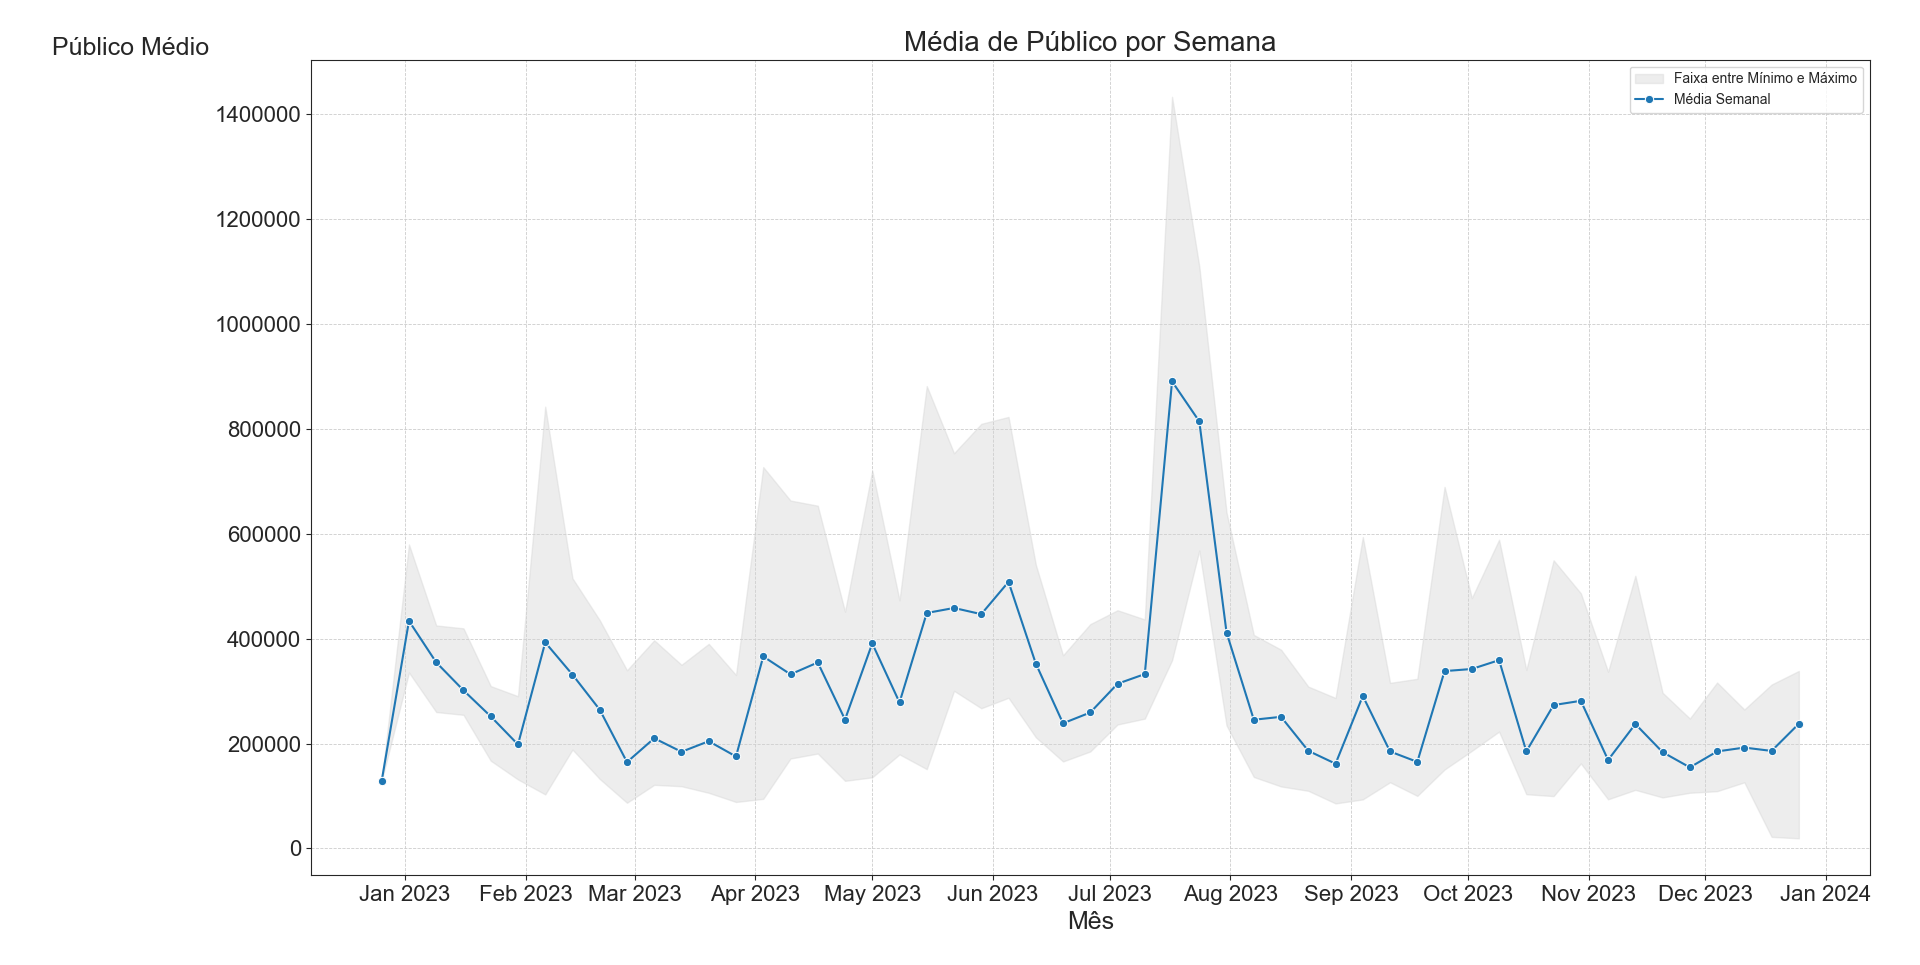
\includegraphics[width = \linewidth]{img/Figure_1.png}}
\end{figure}

\lipsum[1-2]  
\subsection*{Visualização 2:}
\begin{figure}[H]
    \centerline{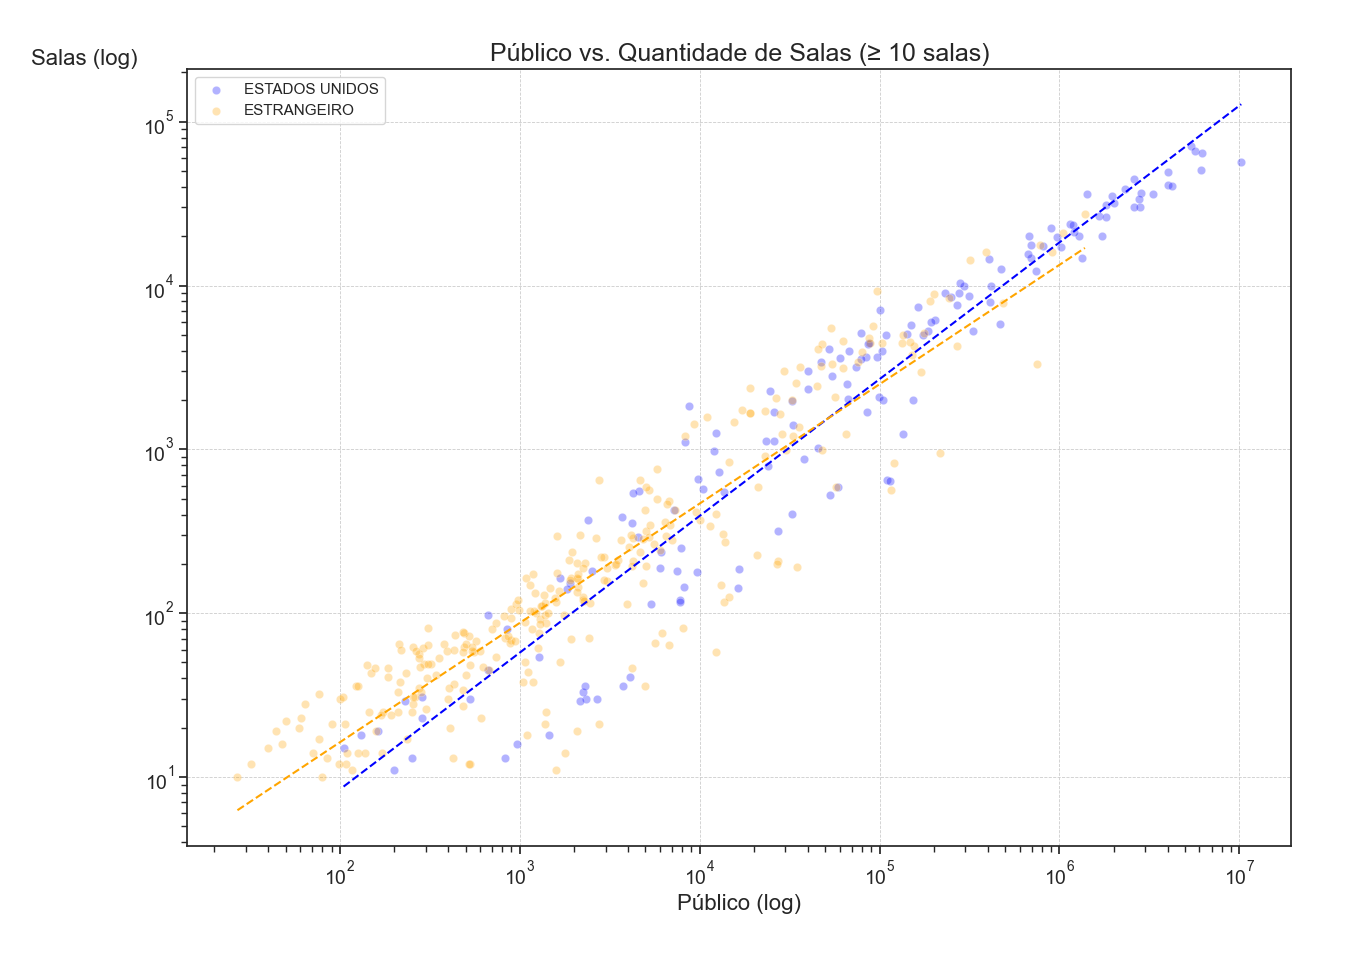
\includegraphics[width = \linewidth]{img/Figure_2.png}}
\end{figure}

O modelo de regressão linear no espaço logarítmico é dado por:

\[
\log_{10}(y) = a \cdot \log_{10}(x) + b
\]

onde:
\begin{itemize}
    \item \(y\) representa a quantidade de salas,
    \item \(x\) representa o público,
    \item \(a\) é o coeficiente angular (inclinação) da reta,
    \item \(b\) é o intercepto da reta.
\end{itemize}

\bigskip

A transformação para o espaço original é dada por:

\[
y = 10^{b} \cdot x^{a}
\]
\[
\min_{a,b} \sum_{i} \left( \log_{10}(y_i) - \left(a \cdot \log_{10}(x_i) + b \right) \right)^2
\]

onde \(\{(x_i, y_i)\}\) são os dados observados com \(x_i, y_i > 0\).

\subsection*{Visualização 3:}
\begin{figure}[H]
    \centerline{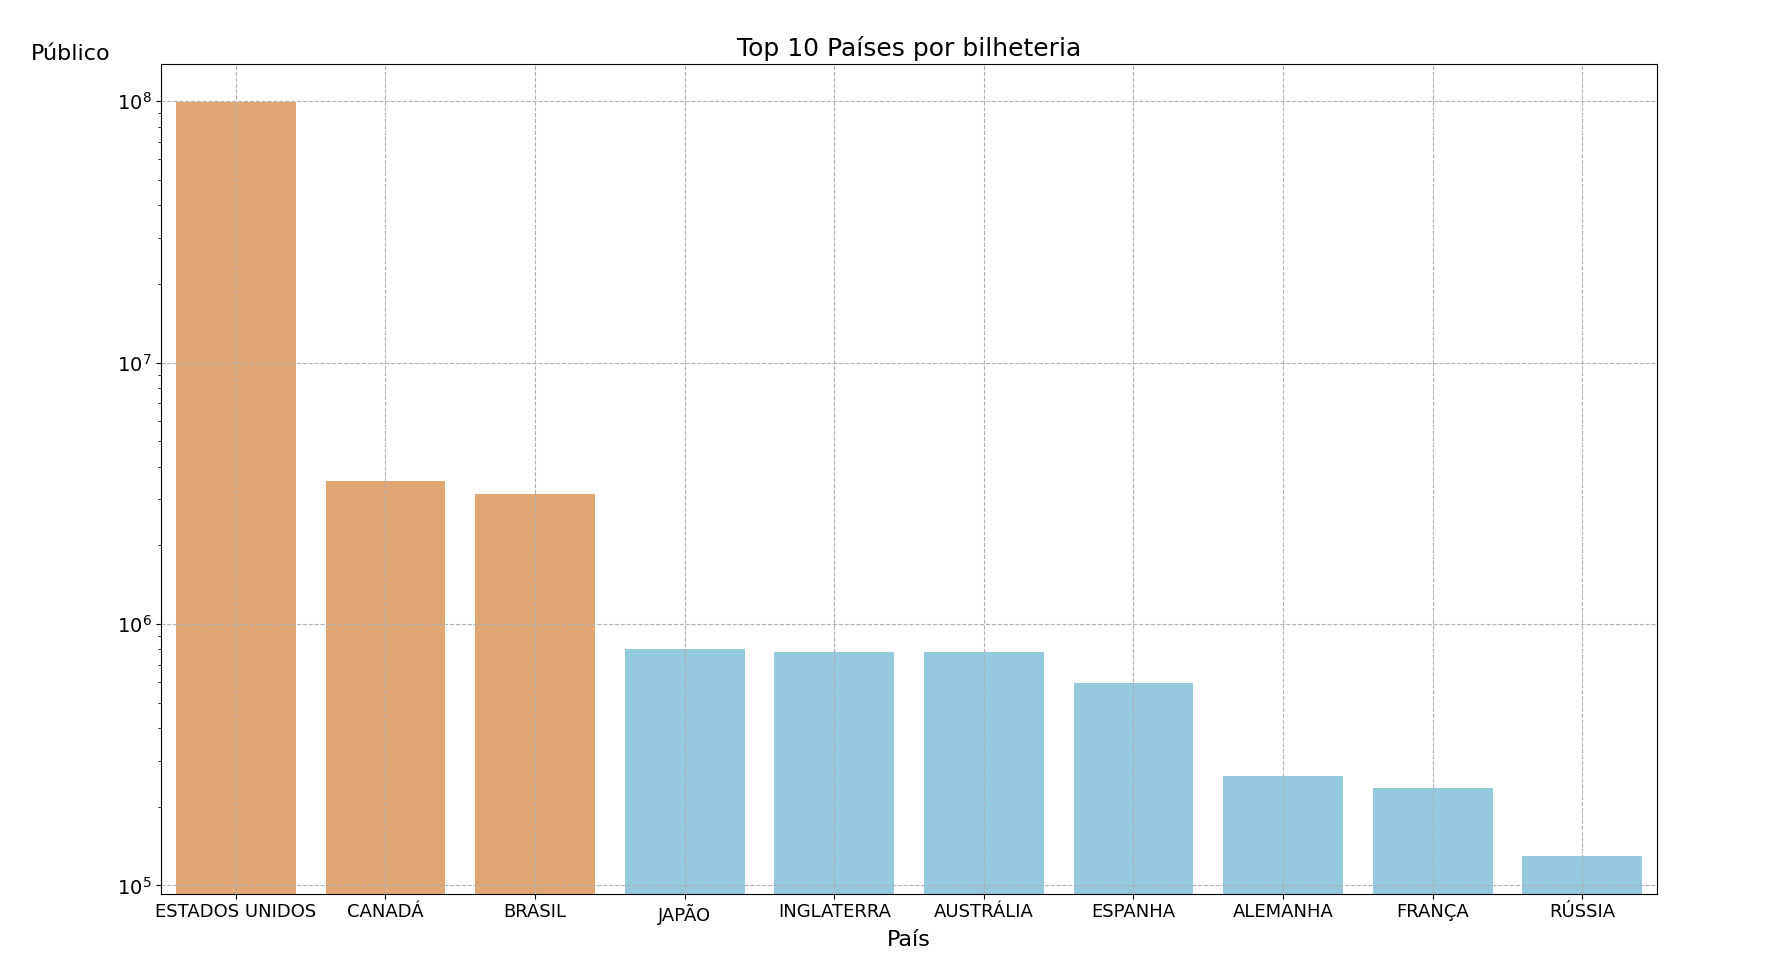
\includegraphics[width = \linewidth]{img/Figure_3.png}}
\end{figure}
\lipsum[1-2]

\subsection*{Visualização 4:}
\begin{figure}[H]
    \centerline{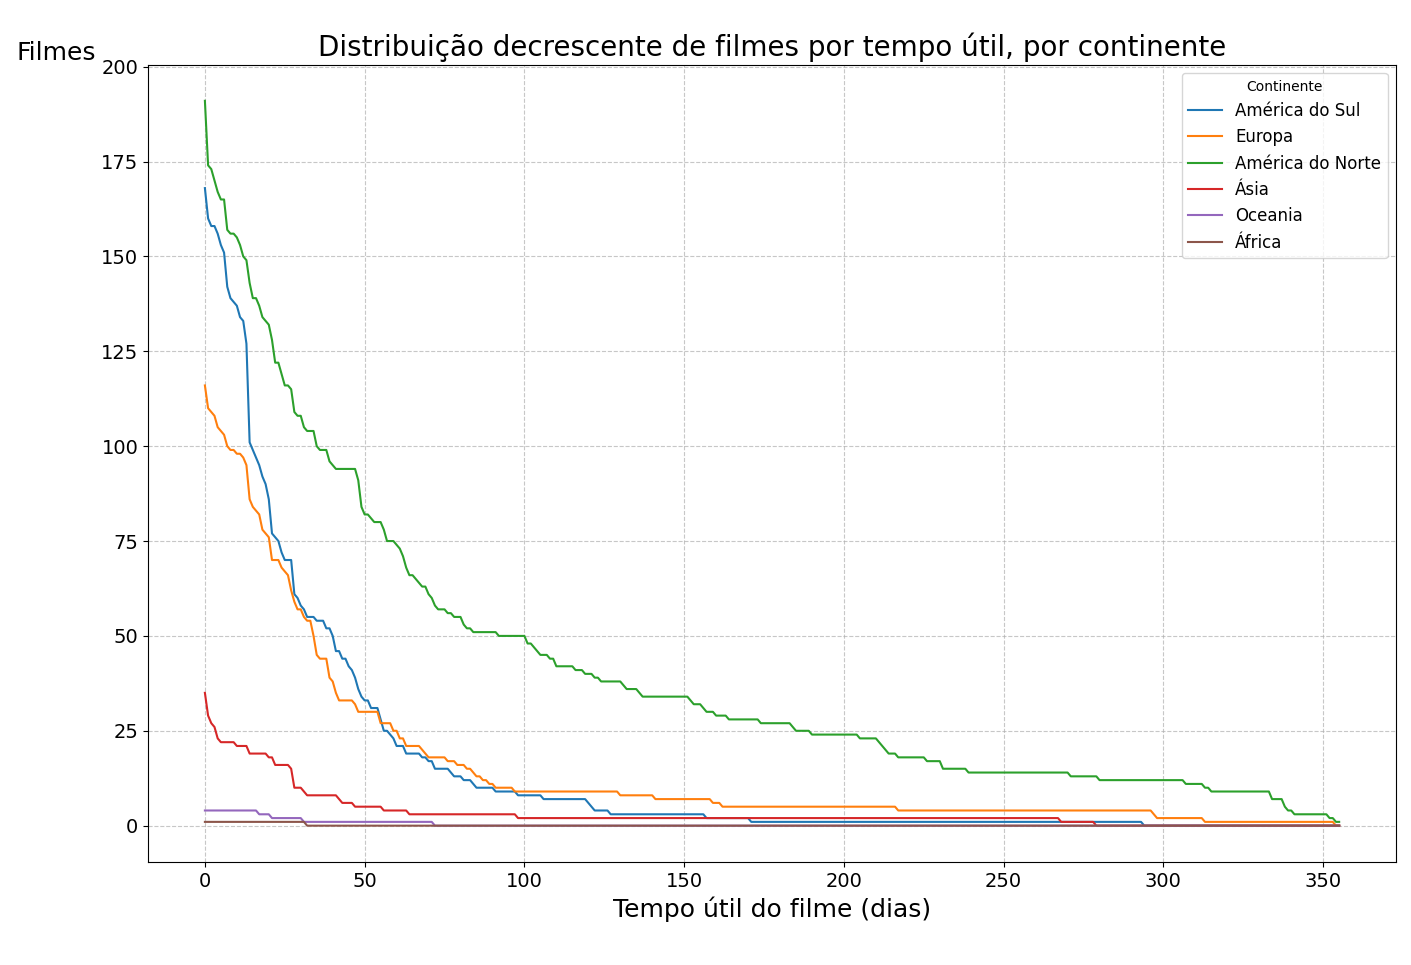
\includegraphics[width = \linewidth]{img/Figure_4.png}}
\end{figure}
\lipsum[1-2]

\section*{Tabelas}
\subsection*{Tabela 1}
\begin{table}[H]
\centering
\caption{Tempo útil médio de exibição por país de origem}
\begin{tabular}{l r}
\hline
\textbf{País de Origem} & \textbf{Tempo Útil Médio (dias)} \\
\hline
SUÉCIA & 161.00 \\
CHINA & 143.75 \\
BELARUS (BIELORUSSIA) & 129.00 \\
ESPANHA & 109.60 \\
IRÃ & 97.00 \\
ESTADOS UNIDOS & 75.43 \\
CANADÁ & 75.22 \\
POLÔNIA & 73.60 \\
ÁUSTRIA & 68.00 \\
BÉLGICA & 58.00 \\
COLÔMBIA & 58.00 \\
ALEMANHA & 55.44 \\
EMIRADOS ÁRABES UNIDOS & 55.00 \\
PANAMÁ & 54.00 \\
HOLANDA & 41.00 \\



\end{tabular}
\begin{center}
\ldots
\end{center}
\end{table}
\subsection*{Tabela 2}
\begin{table}[H]
\centering
\caption{Estatísticas de público por filme: média, desvio padrão e moda do dia da semana}
\begin{tabularx}{\textwidth}{X r r l}
\hline
\textbf{Título} & \textbf{Média de Público} & \textbf{Desvio Padrão} & \textbf{Moda Dia} \\
\hline
FALE COMIGO & 227.83 & 299.91 & Quinta-feira \\
GODZILLA MINUS ONE & 227.07 & 216.66 & Quinta-feira \\
DECISÃO DE PARTIR & 211.83 & 231.45 & Quinta-feira \\
13 EXORCISMOS & 205.23 & 154.26 & Quinta-feira \\
BARBIE & 181.65 & 241.66 & Sábado \\
TRIÂNGULO DA TRISTEZA & 180.03 & 208.68 & Quinta-feira \\
THE CHOSEN - OS ESCOLHIDOS - TEMPORADA 4 - PARTE 1 & 179.42 & 102.65 & Quinta-feira \\
TUDO EM TODO O LUGAR AO MESMO TEMPO & 169.97 & 197.06 & Quinta-feira \\
SAPATINHO VERMELHO E OS SETE ANÕES & 161.00 & --- & Quinta-feira \\
ENCANTO & 160.00 & --- & Quarta-feira \\



\end{tabularx}
\begin{center}
$\ldots$
\end{center}
\end{table}


\begin{thebibliography}{99}

\bibitem{ref1}
Autor, A. (Ano). \textit{Título do Livro}. Editora.

\end{thebibliography}

\end{document}
